\documentclass[12pt]{article}
\usepackage{fullpage}
\usepackage[utf8]{inputenc}
\usepackage{pict2e}
\usepackage{amsmath}
\usepackage{enumitem}
\usepackage{eurosym}
\usepackage{pict2e}
\usepackage{mathtools}
\usepackage{amssymb, amsfonts, latexsym, cancel}
\setlength{\parskip}{0.3cm}
\usepackage{graphicx}
\usepackage{fontenc}
\usepackage{slashbox}
\usepackage{setspace}
\usepackage{gensymb}
\usepackage{accents}
\usepackage{adjustbox}
\setstretch{1.5}
\usepackage{bold-extra}
\usepackage[document]{ragged2e}
\usepackage{subcaption}
\usepackage{tcolorbox}
\usepackage{xcolor, colortbl}
\usepackage{wrapfig}
\usepackage{empheq}
\usepackage{array}
\usepackage{parskip}
\usepackage{arydshln}
\graphicspath{ {images/} }
\renewcommand*\contentsname{\color{black}Índice} 
\usepackage{array, multirow, multicol}
\definecolor{lightblue}{HTML}{007AFF}
\usepackage{color}
\usepackage{etoolbox}
\usepackage{listings}
\usepackage{mdframed}
\setlength{\parindent}{0pt}
\usepackage{underscore}
\usepackage{hyperref}
\usepackage{tikz}
\usepackage{tikz-cd}
\usetikzlibrary{shapes, positioning, patterns}
\usepackage{tikz-qtree}
\usepackage{biblatex}
\usepackage{pdfpages}
\usepackage{pgfplots}
\usepackage{pgfkeys}
\addbibresource{biblatex-examples.bib}
\usepackage[a4paper, left=1.5cm, right=1.5cm, top=1cm,
bottom=1.5cm]{geometry}
\everymath{\displaystyle}
\usetikzlibrary{decorations.pathreplacing}
\usepackage{titlesec}
\usepackage{titletoc}
\usepackage{tikz-3dplot}
\usetikzlibrary{decorations.pathreplacing}
\newcommand{\Ej}{\textcolor{lightblue}{\underline{Ejemplo}}}
\setlength{\fboxrule}{1.5pt}
\renewcommand{\arraystretch}{1.35}
\setlength{\arraycolsep}{0.3cm}

% Configura el formato de las secciones utilizando titlesec
\titleformat{\section}
{\color{red}\normalfont\LARGE\bfseries}
{Tema \thesection:}
{10 pt}
{}

% Ajusta el formato de las entradas de la tabla de contenidos
\addtocontents{toc}{\protect\setcounter{tocdepth}{4}}
\addtocontents{toc}{\color{black}}

\titleformat{\subsection}
{\normalfont\Large\bfseries\color{red}}{\thesubsection)}{1em}{\color{lightblue}}

\titleformat{\subsubsection}
{\normalfont\large\bfseries\color{red}}{\thesubsubsection)}{1em}{\color{lightblue}}

\newcommand{\bboxed}[1]{\fcolorbox{lightblue}{lightblue!10}{$#1$}}

\DeclareMathOperator{\N}{\mathbb{N}}
\DeclareMathOperator{\Z}{\mathbb{Z}}
\DeclareMathOperator{\R}{\mathbb{R}}
\DeclareMathOperator{\Q}{\mathbb{Q}}
\DeclareMathOperator{\K}{\mathbb{K}}
\DeclareMathOperator{\im}{\imath}
\DeclareMathOperator{\jm}{\jmath}
\DeclareMathOperator{\col}{\mathrm{Col}}
\DeclareMathOperator{\fil}{\mathrm{Fil}}
\DeclareMathOperator{\rg}{\mathrm{rg}}
\DeclareMathOperator{\nuc}{\mathrm{nuc}}
\DeclareMathOperator{\dimf}{\mathrm{dimFil}}
\DeclareMathOperator{\dimc}{\mathrm{dimCol}}
\DeclareMathOperator{\dimn}{\mathrm{dimnuc}}
\DeclareMathOperator{\dimr}{\mathrm{dimrg}}

\newcommand{\bu}[1]{\textcolor{lightblue}{\underline{#1}}}
\newcommand{\lb}[1]{\textcolor{lightblue}{#1}}
\newcommand{\db}[1]{\textcolor{blue}{#1}}
\newcommand{\rc}[1]{\textcolor{red}{#1}}
\newcommand{\tr}{^\intercal}

\renewcommand{\CancelColor}{\color{lightblue}}

\newcommand{\dx}{\:\mathrm{d}x}
\newcommand{\dt}{\:\mathrm{d}t}
\newcommand{\dy}{\:\mathrm{d}y}
\newcommand{\dz}{\:\mathrm{d}z}
\newcommand{\dth}{\:\mathrm{d}\theta}
\newcommand{\dr}{\:\mathrm{d}\rho}
\newcommand{\du}{\:\mathrm{d}u}
\newcommand{\dv}{\:\mathrm{d}v}
\newcommand{\tozero}[1]{\cancelto{0}{#1}}
\newcommand{\lbb}[2]{\textcolor{lightblue}{\underbracket[1pt]{\textcolor{black}{#1}}_{#2}}}
\newcommand{\dbb}[2]{\textcolor{blue}{\underbracket[1pt]{\textcolor{black}{#1}}_{#2}}}
\title{Señales y Sistemas\\Problemas Tema 2: Sistemas Lineales e Invariantes en el Tiempo}

\begin{document}
\maketitle
\begin{enumerate}[label=\color{red}\textbf{\arabic*)}]
  \item \lb{Obtenga la convolución de las señales $x(t)=\prod\left( \dfrac{t-\frac{T}{2} }{T} \right) $ y $h(t)=t\prod\left( \dfrac{t-T}{2T} \right)$.}

    La convolución de las funciones $x(t)$ y $h(t)$ se define como: \[
      y(t)=(x\ast h)(t)=\int_{-\infty}^{\infty} x(\tau) h(t-\tau)\mathrm{d}\tau
    \] 
    Dado que $x(t)$ y  $h(t)$ son funciones de duración finita, la integral se reduce al intervalo donde ambas funciones se superponen.

     \textbf{Paso a paso:}
     \begin{itemize}[label=\textbullet]
       \item \textbf{Intervalo de integración:}

         La convolución será no nula solo en el intervalo donde las funciones se superponen. Dado que $x(t)$ está definido en  $[0,T]$ y  $h(t)$ en  $[0,2T]$, la convolución  $y(t)$ será no nula en el intervalo $[0,3T]$.
       \item  \textbf{Evaluación de la integral:}

         Para cada $t$ en  $[0,3T]$, evaluamos la integral:  \[
           y(t)=\int_{0}^{T} \prod\left( \dfrac{\tau-\frac{T}{2}}{T} \right)  (t-\tau)\prod\left( \dfrac{t-\tau-T}{2T} \right) \mathrm{d}\tau.
         \] 
         Simplificando las funciones rectangulares, la integral se reduce a: \[
         y(t)=\int_{\max(0,t-2T)}^{\min(T,t)}(t-\tau)\mathrm{d}\tau.
         \] 
       \item \textbf{Cálculo de la integral:}

         Evaluamos la integral en los intervalos donde las funciones se superponen:
         \begin{itemize}[label=\textbullet]
           \item Para $0\le t<T$, la integral es: \[
           y(t)=\int_{0}^{t} (t-\tau)\mathrm{d}\tau=\left[ t\tau-\dfrac{\tau^2}{2} \right] _0^t=\dfrac{t^2}{2} 
           \] 
           \item Para $T\le t<2T$, la integral es: \[
         y(t)=\int_{0}^{T} (t-\tau)\mathrm{d}\tau=\left[ t\tau-\dfrac{\tau^2}{2} \right] _0^T=tT-\dfrac{T^2}{2} 
         \] 
           \item Para $2T\le t<3T$, la integral es: \[
           y(t)=\int_{t-2T}^{T} (t-\tau)\mathrm{d}\tau =\left[ t\tau-\dfrac{\tau^2}{2} \right] _{t-2T}^{T}=\dfrac{(3T-t)^2}{2}
           \] 
           La convolución $y(t)$ es:  \[
           y(t)=\begin{cases}
             \dfrac{t^2}{2}, & 0\le t<T\\
             tT-\dfrac{T^2}{2}, & T\le t<2T\\
             \dfrac{(2T-t)^2}{2}, & 2T\le t\le 3T\\
             0, & \text{en otro caso}
           \end{cases}
           \] 
         \end{itemize}
     \end{itemize}
  \item \lb{Calcule $\left( \dfrac{t}{T_1}+1 \right)\prod\left( \dfrac{t-\frac{T_1}{2} }{T_1} \right) \ast\prod\left( \dfrac{t-\frac{T_2}{2} }{T_2} \right)  $, con $T_2>T_1$.} 

    \begin{enumerate}[label=Paso \arabic*:]
      \item Comprender las señales
        \begin{itemize}[label=\textbullet]
          \item Primera señal: \[
          x(t)=\left( \dfrac{t}{T_1}+1 \right) \prod\left( \dfrac{t-\frac{T_1}{2} }{T_1} \right)
          \] 
          \begin{itemize}[label=\textbullet]
            \item La función $\prod\left( \dfrac{t-\frac{T_1}{2} }{T_1} \right) $ es una función rectangular centrada en $t=\dfrac{T_1}{2}$ con un ancho de $T_1$. Esto significa que $\prod$ es igual a 1 en el intervalo  $[0,T_1]$ y 0 fuera de este intervalo.
            \item Por lo tanto, $x(t)$ es una función lineal definida únicamente $[0,T_1]$, con: \[
                x(t)=\dfrac{t}{T_1}+1,\quad\text{para }t\in [0,T_1].
            \] 
            \begin{center}
              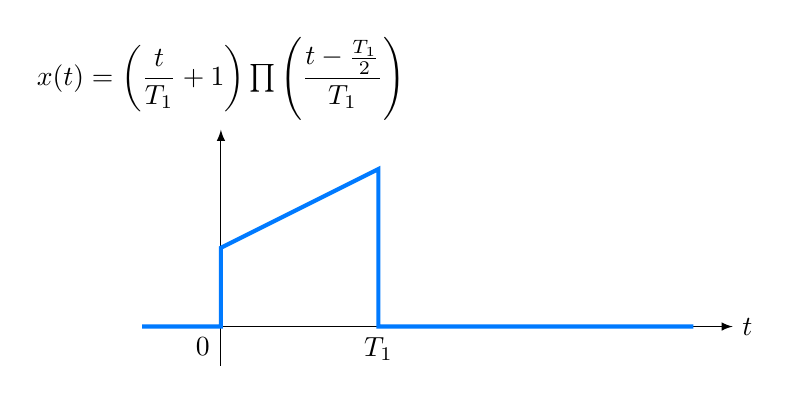
\begin{tikzpicture}[>=latex]
                \draw[->] (-1, 0) -- (6.5,0) node[right] {$t$};
                \draw[->] (0,-0.5) -- (0, 2.5) node[above] {$x(t)=\left( \dfrac{t}{T_1}+1 \right ) \prod\left( \dfrac{t-\frac{T_1}{2} }{T_1} \right )$};
                \draw[lightblue, line width=1.5] (-1,0) -- (0,0) node[below left, black] {$0$} -- (0,1) -- (2,2) -- (2,0) node[below, black] {$T_1$} -- (6,0);
              \end{tikzpicture}
            \end{center}
          \end{itemize}
        \item Segunda señal: \[
        h(t)=\prod\left( \dfrac{t-\frac{T_2}{2} }{T_2} \right) .
        \] 
        \begin{itemize}[label=\textbullet]
          \item Esta es una función rectangular centrada en $t=\dfrac{T_2}{2}$ con un ancho de $T_2$. Es igual a 1 en el intervalo $[0,T_2]$ y 0 fuera de este intervalo.
            \begin{center}
              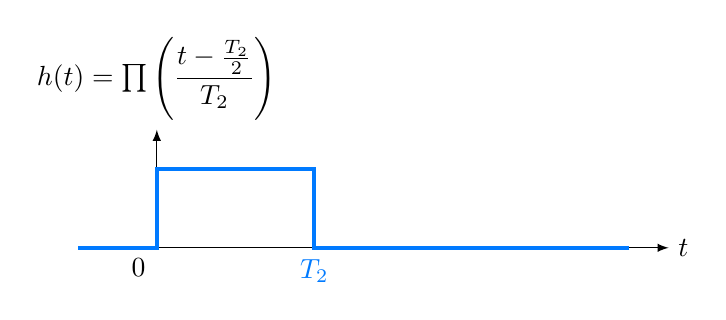
\begin{tikzpicture}[>=latex]
                \draw[->] (-1,0) -- (6.5,0) node[right] {$t$};
                \draw[->] (0,0.5) -- (0,1.5) node[above] {$h(t)=\prod\left( \dfrac{t-\frac{T_2}{2} }{T_2} \right )$};
                \draw[lightblue, line width=1.5] (-1,0) -- (0,0) node[below left, black] {$0$} -- (0,1) -- (2,1) -- (2,0) node[below] {$T_2$} -- (6,0);
              \end{tikzpicture}
            \end{center}
        \end{itemize}
      \item Convolución de las señales

        La convolución de $x(t)$ y  $h(t)$ se define como:  \[
        y(t)=(x\ast h)(t)=\int_{-\infty}^{\infty} x(\tau)h(t-\tau) \mathrm{d}\tau.
        \] 
        Dado que $x(t)$ está definido en  $[0,T_1]$ y $h(t)$ en  $[0,T_2]$, la convolución será no nula únicamente en el intervalo donde ambas funciones se superponen. Esto ocurre en el intervalo $[0,T_1+T_2]$.

        \textbf{Intervalo de integración:}
        \begin{itemize}[label=\textbullet]
          \item Para cada $t\in [0,T_1+T_2]$, la integral se reduce a: \[
          y(t)=\int_{\max(0,t-T_2)}^{\min(T_1,t)}  x(\tau)\mathrm{d}\tau,
        \] ya que $h(t-\tau)$ es no nula cuando  $t-\tau\in [0,T_2]$, es decir, $\tau\in [t-T_2,t]$, y $x(\tau)$ es no nula solo cuando  $\tau\in (0,T_1)$.
        \end{itemize}
        \end{itemize}
      \item Evaluar la integral

        En el interalo de integración, $x(\tau)=\dfrac{\tau}{T_1}+1$. Sustituyendo esto en la integral: \[
          \begin{aligned}
          y(t)=\int_{\max(0,t-T_2)}^{\min(T_1,t)} \left( \dfrac{\tau}{T_1}+1 \right) \mathrm{d}\tau&=\int_{\max(0,t-T_2)}^{\min(T_1,t)} \dfrac{\tau}{T_1}\mathrm{d}\tau+\int_{\max(0,t-T_2)}^{\min(T_1,t)} 1\mathrm{d}\tau\\ &=\bboxed{\dfrac{1}{T_1}\left( \dfrac{\min(T_1,t)^2}{2}-\dfrac{\max(0,t-T_2)^2}{2} \right ) +\min(T_1,t)-\max(0,t-T_2)} 
          \end{aligned}
        \] 
         \begin{itemize}[label=\textbullet]
           \item $\int_{\max(0,t-T_2)}^{\min(T_1,t)} \dfrac{\tau}{T_1}\mathrm{d}\tau=\dfrac{1}{T_1}\int_{\max(0,t-T_2)}^{\min(T_1,t)} \tau\mathrm{d}\tau=\dfrac{1}{T_1}\left[ \dfrac{\tau^2}{2} \right]_{\max(0,t-T_2)}^{\min(T_1,t)}=\dfrac{1}{T_1}\left( \dfrac{\min(T_1,t)^2}{2}-\dfrac{\max(0,t-T_2)^2}{2} \right)  $.
           \item $\int_{\max(0,t-T_2)}^{\min(T_1,t)} 1\mathrm{d}\tau = [\tau]_{\max(0,t-T_2)}^{\min(T_1,t)} =\min(T_1,t)-\max(0,t-T_2)$
        \end{itemize}
    \end{enumerate}
  \item \lb{Calcule la convolución de $x(t)=e^{2t}u(-t)$ con $h(t)=u(t-3)$.}

    La convolució se define como: \[
    y(t)=(x\ast h)(t)=\int_{-\infty}^{\infty} x(\tau)h(t-\tau)\mathrm{d}\tau 
    \] 
    \textbf{Análisis de las señales}
    \begin{itemize}[label=\textbullet]
      \item $x(t)=e^{2t}u(-t) $ es una señal exponencial que existe solo para $t<0$.
      \item  $h(t)=u(t-3)$ es un escalón unitario desplazado 3 unidades a la derecha.
    \end{itemize}
    \begin{center}
      \begin{tikzpicture}
          \begin{axis}[
              width=7.5cm,
              height=6cm,
              axis lines=middle,
              xlabel={$t$},
              ylabel={$x(t)$},
              ymin=-0.1, ymax=1.1,
              axis line style={-},
              every axis plot/.append style={thick, lightblue}
          ]
              \addplot[
                  domain=-2:6,
                  samples=1000
              ]
              {exp(2*x)*(x<=0)};
          \end{axis}
      \end{tikzpicture}\qquad
      \begin{tikzpicture}
          \begin{axis}[
              width=7.5cm,
              height=6cm,
              axis lines=middle,
              xlabel={$t$},
              ylabel={$h(t)$},
              ymin=-0.1, ymax=1.1,
              axis line style={-},
              every axis plot/.append style={thick, lightblue},
              x label style={at={(current axis.right of origin)}}
          ]
              \addplot[
                  domain=-2:6,
                  samples=1000
              ]
              {x>=3 ? 1 : 0};
          \end{axis}
      \end{tikzpicture}
    \end{center}
    \textbf{Determinación de los límites de integración}
    
    Para que la integral no sea nula, necesitamos que:
    \begin{itemize}[label=\textbullet]
      \item $\tau<0$ (debido a $u(-\tau)$ en  $x(\tau)$) 
      \item $t-\tau>3$ (debido a $u(t-\tau-3)$ en  $h(t-\tau)$)
    \end{itemize}
    De $t-\tau>3$, obtenemos:  $\tau<t-3$. Por tanto, los límites de itengración son:
     \begin{itemize}[label=\textbullet]
      \item Límite inferior: $-\infty$
      \item Límite superior: $\min(0,t-3)$
    \end{itemize}
    \textbf{Cálculo de la convolución}
    \[
    y(t)=\int_{-\infty}^{\min(0,t-3)} e^{2\tau}(u-\tau)u(t-\tau-3)\mathrm{d}\tau 
    \] 
    Debemos considerar dos casos:
    \begin{enumerate}[label=Caso \arabic*:]
      \item $t<3$

        En este caso,  $t-3<0$, por lo que  $\min(0,t-3)=t-3$
         \[
        y(t)=\int_{-\infty}^{t-3} e^{2\tau}\mathrm{d}\tau=\dfrac{1}{2}e^{2(t-3)}=\dfrac{1}{2}e^{2t-6}    
        \] 
      \item $t\ge 3$

        En este caso, $t-3\ge 0$, por lo que $\min(0,t-3)=0$
         \[
           y(t)=\int_{-\infty}^{0} e^{2\tau}\mathrm{d}\tau=\dfrac{1}{2}
        \] 
        La convolución es: \[
        y(t)=\begin{cases}
          \dfrac{1}{2}e^{2t-6}, & t<3\\
          \dfrac{1}{2}, & t\ge 3
        \end{cases}
        \] 
        \begin{center}
          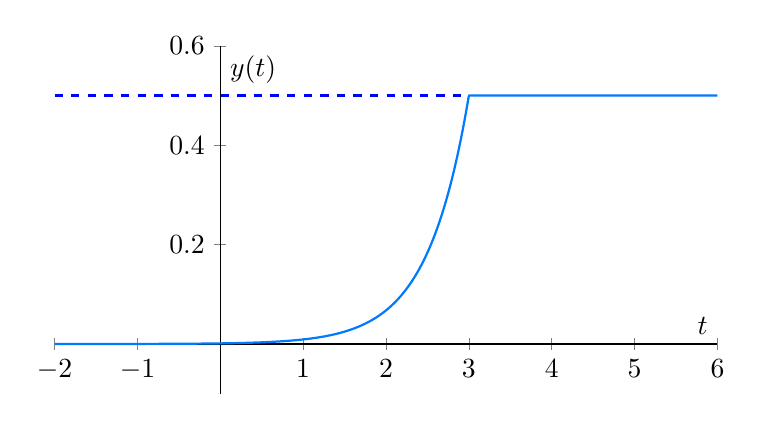
\begin{tikzpicture}
            \begin{axis}[
              width=10cm,
              height=6cm,
              axis lines=middle,
              xlabel={$t$},
              ylabel={$y(t)$},
              axis line style={-},
              ymin=-0.1, ymax=0.6,
              every axis plot/.append style={thick, lightblue}
              ]
              \addplot[domain=-2:6, samples=1000] {x < 3 ? 0.5*exp(2*x-6) : 0.5};
              \addplot[blue, dashed, domain=-2:3, samples=2] {0.5};
            \end{axis} 
          \end{tikzpicture}
        \end{center}
    \end{enumerate}
  \item \lb{Sea $x[n]=\delta[n]+2\delta[n-1]-\delta[n-3]$ y  $h[n]=2\delta[n+1]+2\delta[n-1]$} 
    \begin{center}
      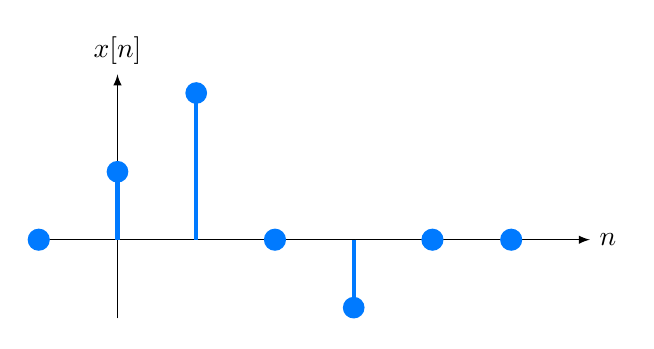
\begin{tikzpicture}[>=latex]
        \draw[->] (-1,0) -- (6,0) node[right] {$n$};
        \draw[->] (0,-1) -- (0,2.1) node[above] {$x[n]$};
        \draw[-*, lightblue, line width=1.5] (0,0) -- (0,1);
        \draw[-*, lightblue, line width=1.5] (1,0) -- (1,2);
        \draw[-*, lightblue, line width=1.5] (3,0) -- (3,-1);
        \foreach \x/\n in {-1/0, 2/0, 4/0, 5/0} {
        \fill[lightblue] (\x,\n) circle (4pt);
        }
      \end{tikzpicture}\qquad
      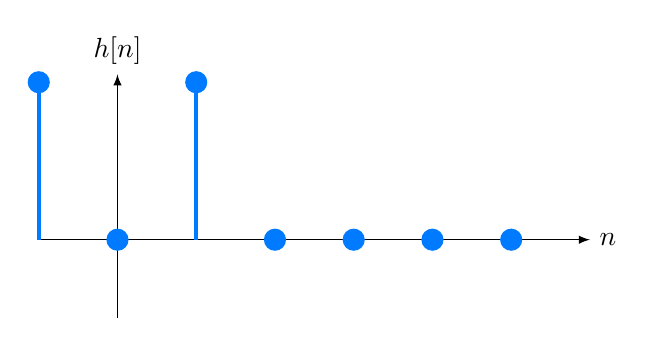
\begin{tikzpicture}[>=latex]
        \draw[->] (-1,0) -- (6,0) node[right] {$n$};
        \draw[->] (0,-1) -- (0,2.1) node[above] {$h[n]$};
        \foreach \x/\n in {-1/2,0/0,1/2,2/0,3/0,4/0,5/0} {
          \fill[lightblue] (\x,\n) circle (4pt);
        }
        \foreach \x in {-1,1} {\draw[lightblue, line width=1.5] (\x,0) -- (\x,2);}
      \end{tikzpicture}
    \end{center}
    \begin{enumerate}[label=\color{red}\textbf{\alph*)}]
      \item \db{$y_1=x[n]\ast h[n]$} 
       
        La convolución se calcula como: \[
          y_1=\sum_{k=-\infty}^{\infty} x[k]h[n-k]
        \] 
        Sustituyendo $x[k]$ y  $h[n-k]$, tenemos: \[
          y_1[n]=x[0]h[n]+x[1]h[n-1]+x[3]h[n-3]
        \] 
         \begin{itemize}[label=\textbullet]
           \item $x[0]=1\longrightarrow h[n]=2\delta[n+1]+2\delta[n-1]$
           \item $x[1]=2\longrightarrow h[n-1]=2\delta[n]+2\delta[n-2]$
           \item $x[3]=-1\longrightarrow h[n-3]=2\delta[n-2]+2\delta[n-4]$
        \end{itemize}
        Sumando todas las contribuciones: \[
          y_1[n]=2\delta[n+1]+2\delta[n-1]+4\delta[n]+4\delta[n-2]-2\delta[n-2]-2\delta[n-4]=2\delta[n+1]+4\delta[n]+2\delta[n-1]+2\delta[n-2]-2\delta[n-4]
        \] 
        \begin{center}
          \begin{tikzpicture}[>=latex]
            \draw[->] (-1,0) -- (6,0) node[right] {$n$};
            \draw[->] (0,-2) -- (0,4.1) node[above] {$y_1[n]$};
            \foreach \x/\n in {-1/2,0/4,1/2,2/2,3/0,4/-2,5/0} {
              \draw (\x, 0.1) -- (\x,-0.1) node[below] {$\x$};
              \draw[line width=1.5, lightblue] (\x,0) -- (\x,\n);
              \fill[lightblue] (\x,\n) circle (3pt);
            }
          \end{tikzpicture}
        \end{center}
      \item \db{$y_2[n]=x[n+2]\ast h[n]$}
        
        Señal desplazada: \[
          x[n+2]=\delta[n+2]+2\delta[n+1]-\delta[n-1]
        \] 
        La convolución se calcula como: \[
          y_2[n]=\sum_{k=-\infty}^{\infty} x[k+2]h[n-k]
        \] 
        Sustituyendo $x[k+2]$ y  $x[n-k]$, tenemos:  \[
          y_2[n]=x[-2]h[n+2]+x[-1]h[n+1]+x[1]h[n-1]
        \] 
        \begin{itemize}[label=\textbullet]
          \item $x[-2]=1\longrightarrow h[n+2]=2\delta[n+3]+2\delta[n+1]$
          \item $x[-1]=2\longrightarrow h[n+1]=2\delta[n+2]+2\delta[n]$
          \item $x[1]=-1\longrightarrow h[n-1]=2\delta[n]+2\delta[n-2]$
        \end{itemize}
        Sumando todas las contribuciones: \[
          y_2[n]=2\delta[n+3]+2\delta[n+1]+4\delta[n+2]+4\delta[n]-2\delta[n]-2\delta[n-2]=2\delta[n+3]+4\delta[n+2]+2\delta[n+1]+2\delta[n]-2\delta[n-2]
        \] 
        \begin{center}
          \begin{tikzpicture}[>=latex]
            \draw[->] (-4,0) -- (5,0) node[right] {$n$};
            \draw[->] (0,-2) -- (0,4.1) node[above] {$y_2[n]$};
            \foreach \x/\n in {-4/0,-3/2,-2/4,-1/2,0/2,1/0,2/-2, 3/0, 4/0} {
              \draw (\x,0.1) -- (\x,-0.1) node[below] {$\x$};
              \draw[line width=1.5, lightblue] (\x,0) -- (\x,\n);
              \fill[lightblue] (\x,\n) circle (3pt);
            }
          \end{tikzpicture}
        \end{center}
      \item \db{$y_3[n]=x[n]\ast h[n+2]$} 

        Señal desplazada: \[
          h[n+2]=2\delta[n+3]+2\delta[n+1]
        \] 
        La convolución se calcula como: \[
          y_3[n]=\sum_{k=-\infty}^{\infty} x[k]h[n-k+2]
        \] 
        Sustituyendo $x[k]$ y $h[n-k+2]$, tenemos:  \[
          y_3[n]=x[0]h[n+2]+x[1]h[n+1]+x[3]h[n-1]
        \] 
        \begin{itemize}[label=\textbullet]
          \item $x[0]=1\longrightarrow h[n+2]=2\delta[n+3]+2\delta[n+1]$
          \item $x[1]=2\longrightarrow h[n+1]=2\delta[n+2]+2\delta[n]$
          \item $x[3]=-1\longrightarrow h[n-1]=2\delta[n]+2\delta[n-2]$
        \end{itemize}
        Sumando todas las contribuciones:
        \[
          y_3[n]=2\delta[n+3]+2\delta[n+1]+4\delta[n+2]+4\delta[n]-2\delta[n]-2\delta[n-2]=2\delta[n+3]+4\delta[n+2]+2\delta[n+1]+2\delta[n]-2\delta[n-2]
        \] 
        \begin{center}
          \begin{tikzpicture}[>=latex]
            \draw[->] (-4,0) -- (5,0) node[right] {$n$};
            \draw[->] (0,-2) -- (0,4.1) node[above] {$y_3[n]$};
            \foreach \x/\n in {-4/0,-3/2,-2/4,-1/2,0/2,1/0,2/-2, 3/0, 4/0} {
              \draw (\x,0.1) -- (\x,-0.1) node[below] {$\x$};
              \draw[line width=1.5, lightblue] (\x,0) -- (\x,\n);
              \fill[lightblue] (\x,\n) circle (3pt);
            }
          \end{tikzpicture}

        \end{center}
    \end{enumerate}
  \item \lb{Un sistema lineal $S$ relaciona su entrada  $x[n]$ y su salida $y[n]$ como \[
        y[n]=\sum_{k=-\infty}^{\infty} x[k]g[n-2k]
    \] donde $g[n]=u[n]-u[n-4]$.} 
    \begin{enumerate}[label=\color{red}\textbf{\alph*)}]
      \item \db{Determine $y[n]$ cuando $x[n]=\delta[n-1]$} 

        La relación entre la entrada y la salida está dada por: \[
          y[n]=\sum_{k=-\infty}^{\infty} x[k]g[n-2k]
        \] 
        Sustituyendo $x[n]=\delta[n-1]$, sabemos que  $\delta[n-1]$ es no nula cuando  $n=1$. Por lo tanto, la suma se reduce a:  \[
          y[n]=g[n-2(1)]=g[n-2]
        \] 
        Dado que $g[n]=u[n]-u[n-4]$, tenemos:  \[
          g[n-2]=u[n-2]-u[n-6]
        \] 
        Por lo tanto: \[
          y[n]=u[n-2]-u[n-6]
        \] 
        Esto significa que $y[n]$ es un pulso rectangular que comienza en  $n=2$ y termina en  $n=5$ (ya que $u[n-6]$) se activa en $n=6$.
         \begin{center}
           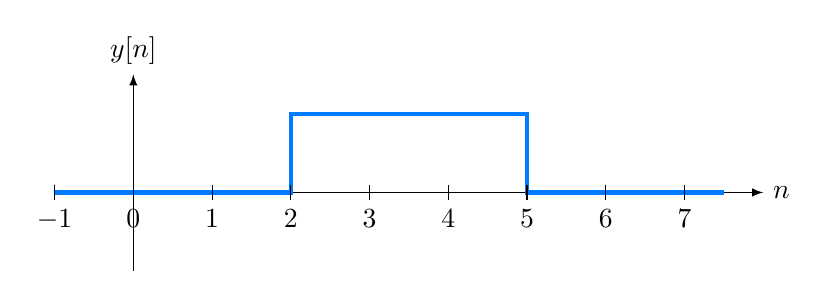
\begin{tikzpicture}[>=latex]
            \draw[->] (-1,0) -- (8,0) node[right] {$n$};
            \draw[->] (0,-1) -- (0,1.5) node[above] {$y[n]$};
            \draw[lightblue, line width=1.5] (-1,0) -- (2,0) -- (2,1) -- (5,1) -- (5,0) -- (7.5,0); 
            \foreach \x in {-1,0,...,7} {\draw (\x,0.1) -- (\x,-0.1) node[below] {$\x$};}
          \end{tikzpicture}
        \end{center}
      \item \db{Determine $y[n]$ cuando $x[n]=\delta[n-2]$} 

        De nuevo, la relación es: \[
          y[n]=\sum_{k=-\infty}^{\infty} x[k]g[n-2k]
        \] 
        Sustituyendo $x[n]=\delta[n-2]$, sabemos que  $\delta[n-2]$ es no nula solo cuando  $n=2$. Por lo tanto, la suma se reduce a: \[
          y[n]=g[n-2(2)]=g[n-4]
        \] 
        Dado que $g[n]=u[n]-u[n-4]$, tenemos:  \[
          g[n-4]=u[n-4]-u[n-8]
        \] 
        Esto significa que $y[n]$ es un pulso rectangular que comienza en $n=4$ y termina en $n=7$ (ya que $u[n-8]$ se activa en $n=8$)
        \begin{center}
           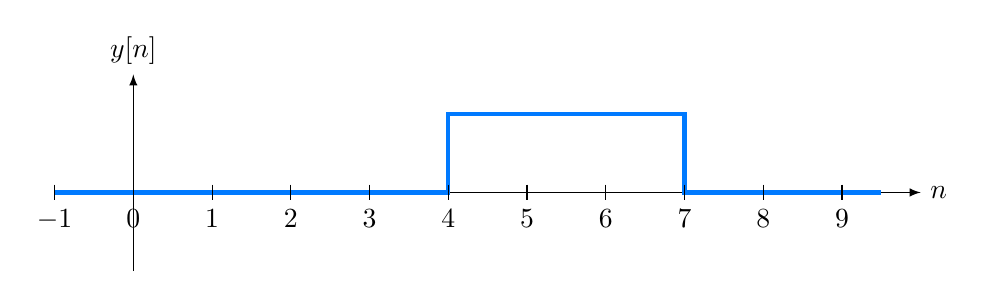
\begin{tikzpicture}[>=latex]
            \draw[->] (-1,0) -- (10,0) node[right] {$n$};
            \draw[->] (0,-1) -- (0,1.5) node[above] {$y[n]$};
            \draw[lightblue, line width=1.5] (-1,0) -- (4,0) -- (4,1) -- (7,1) -- (7,0) -- (9.5,0); 
            \foreach \x in {-1,0,...,9} {\draw (\x,0.1) -- (\x,-0.1) node[below] {$\x$};}
          \end{tikzpicture}
        \end{center}

      \item \db{¿Es $S$ un sistema LTI?} 

        Para determinar si el sitema es \textbf{lineal} e \textbf{invariante} en el tiempo, evaluamos cada propiedad:
        \begin{itemize}[label=\textbullet]
          \item \textbf{Linealidad:}

            Un sistema es lineal si satisface el principio de superposición, es decir, si para dos entradas $x_1[n]$ y $x_2[n]$ con salidas $y_1[n]$ y $y_2[n]$, respectivamente, se cumple que: \[
              S \{ax_1[n]+bx_2[n]\} =ay_1[n]+by_2[n]
            \] 
            En este caso, la salida está dada por una suma ponderada de $x[k]$ y  $g[n-2k]$, lo cual es una operación lineal. Por lo tanto, el sistema es  \textbf{lineal}.
          \item \textbf{Invanrianza en el tiempo:}

            Un sistema es invariante en el tiempo si un desplazamiento en la entrada produce el mismo desplazamiento en la salida. Es decir, si para una entrada $x[n]$ con salida  $y[n]$, al desplazar la entrada  $x[n-n_0]$, la salida se desplaza de manera idéntica $y[n-n_0]$.

            En este caso, la salida depende de $g[n-2k]$, que introduce un factor de escalamiento en el índice  $k$. Esto significa que el sistema  \textbf{no es invariante en el tiempo}, ya que el desplazamiento de la entrada no se traduce directamente en un desplazamiento de la salida. 
        \end{itemize}
      \item \db{Determine $y[n]$ cuando $x[n]=u[n]$} 

        De nuevo, la relación es: \[
          y[n]=\sum_{k=-\infty}^{\infty} x[k]g[n-2k]
        \] 
        Sustituyendo $x[n]=u[n]$, sabemos que  $u[n]$ es no nula para  $k\ge 0$. Por lo tanto, la suma se reduce a: \[
          y[n]=\sum_{k=0}^{\infty} g[n-2k]
        \] 
        Dado que $g[n]=u[n]-u[n-4]$, tenemos:  \[
          g[n-2k]=u[n-2k]-u[n-2k-4]
        \] 
        Sustituyendo esto en la suma: \[
          y[n]=\sum_{k=0}^{\infty} (u[n-2k]-u[n-2k-4])
        \] 
        La suma se puede interpretar como una superposición de pulsos rectangulares desplazados. Cada término $u[n-2k]-u[n-2k-4]$ es un pulso rectangular de longitud 4, comenzando en  $n=2k$ y terminando en  $n=2k+3$.

        Por lo tanto,  $y[n]$ es una secuencia de pulsos rectangulares de longitud 4, comenzando en  $n=0$ y repitiéndose cada 2 unidades de tiempo.
         \begin{center}
           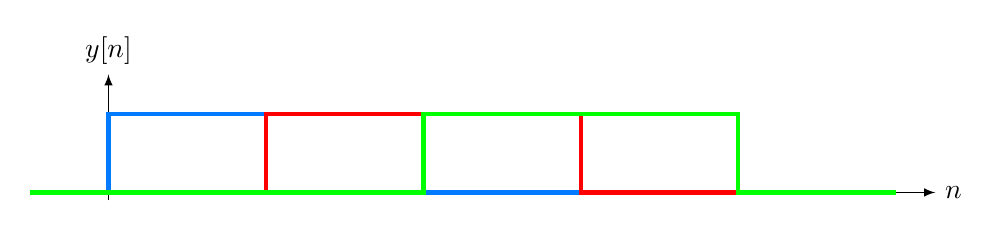
\begin{tikzpicture}[>=latex]
            \draw[->] (-1,0) -- (10.5,0) node[right] {$n$};
            \draw[->] (0,-0.1) -- (0, 1.5) node[above] {$y[n]$};
            \draw[lightblue, line width=1.5] (-1,0) -- (0,0) -- (0,1) -- (4,1) -- (4,0) -- (10, 0);
            \draw[red, line width=1.5] (-1,0) -- (2,0) -- (2,1) -- (6,1) -- (6,0) -- (10, 0);
            \draw[green, line width=1.5] (-1,0) -- (4,0) -- (4,1) -- (8,1) -- (8,0) -- (10, 0);
          \end{tikzpicture}
        \end{center}
    \end{enumerate}
  \item \lb{Determine y esboce la convolución de las siguientes señales: \[
  \begin{array}{cc}
    x(t)=\begin{cases}
      t+1, & 0\le t\le 1\\
      2-t, & 1<t\le 2\\
      0, & \text{otro valor}
    \end{cases} & h(t)=\delta(t+2)+2\delta(t+1)
  \end{array}
\] }
La convolución de dos señales $x(t)$ y  $h(t)$ está definida como:  \[
y(t)=(x\ast h)(t)=\int_{-\infty}^{\infty} h(\tau)h(t-\tau)\mathrm{d}\tau 
\] 
En este caso:
\begin{itemize}[label=\textbullet]
  \item $x(t)$ es una función triangular definida por tramos:  \[
  x(t)=\begin{cases}
    t+1, & 0\le t\le 1\\
    2-t, & 1<t\le 2\\
    0, & \text{en otro caso}
  \end{cases}
  \] 
\item $h(t)$ es una combinación de deltas desplazadas:  \[
h(t)=\delta(t+2)+2\delta(t+1)
\] 
\end{itemize}
Dado que $h(t)$ está compuesto por deltas, la convolución se simplifica porque las deltas actúan como "muestradoras" de  $x(t)$. Específicamente, la convolución se convierte en:  \[
y(t)=x(t)\ast h(t)=x(t+2)+2x(t+1)
\] 
\begin{enumerate}[label=Paso \arabic*:]
  \item Determinar $x(t+2)$

    Para obtener  $x(t+2)$, desplazamos  $x(t)$ dos unidades hacia la izquierda. Esto significa que el soporte de  $x(t+2)$ (el intervalo donde es cero) será:  \[
    -2\le t\le -1
    \] 
    En este intervalo, la forma de $x(t+2)$ es: 
    \begin{itemize}[label=\textbullet]
      \item Para $-2\le t\le -1,x(t+2)=t+2+1=t+3$.
    \end{itemize}
    Por lo tanto: \[
    x(t+2)=\begin{cases}
      t+3, & -2\le t\le -1\\
      0, & \text{en otro caso}
    \end{cases}
    \] 
  \item Determinar $2x(t+1)$

    Para obtener  $2x(t+1)$, desplazamos  $x(t)$ una unidad hacia la izquierda y multiplicamos por 2. Esto significa que el soporte de  $2x(t+1)$ será:  \[
    -1\le t\le 1
    \] 
    En este intervalo, la forma de $x(t+1)$ es:
     \begin{itemize}[label=\textbullet]
      \item Para $-1\le t\le 0,x(t+1)=t+1+1=t+2$
      \item Para $0<t\le 1,x(t+1)=2-(t-1)=1-t$
    \end{itemize}
    Multiplicando por 2, obtenemos: \[
    2x(t+1)=\begin{cases}
      2(t+2)=2t+4, & -1\le t\le 0\\
      2(1-t)=2-2t, & 0<t\le 1\\
      0, & \text{en otro caso}
    \end{cases}
    \] 
  \item Sumar $x(t+2)$ y  $2x(t+1)$

    Ahora sumamos las dos contribuciones  $x(t+2)$ y  $2x(t+1)$. El soporte total de $y(t)$ será la unión de los soportes de  $x(t+2)$ y  $2x(t+1)$, es decir:  \[
    -2\le t\le 1
    \] 
    Dividimos el cálculo en intervalos:
    \begin{itemize}[label=\textbullet]
      \item Para $-2\le t<-1$:
        \begin{itemize}[label=\textbullet]
          \item $x(t+2)=t+3$
          \item  $2x(t+1)=0$ (porque $t+1<-1$) 
          \item $y(t)=t+3$
        \end{itemize}
      \item Para $-1\le t<0$:
        \begin{itemize}[label=\textbullet]
          \item $x(t+2)=t+3$
          \item  $2x(t+1)=2t+4$
          \item  $y(t)=(t+3)+(2t+4)=3t+7$
        \end{itemize}
      \item Para $0\le t\le 1$:
        \begin{itemize}[label=\textbullet]
          \item $x(t+2)=0$ (porque $t+2>2$) 
          \item $2x(t+1)=2-2t$
          \item  $y(t)=0+(2-2t)=2-2t$
        \end{itemize}
    \end{itemize}
\end{enumerate}
    La salida $y(t)$ es:  \[
    y(t)=\begin{cases}
      t+3, & -2\le t<-1\\
      3t+7, & -1\le t<0\\
      2-2t, & 0\le t<1\\
      0, & \text{en otro caso}
    \end{cases}
    \]
    \begin{center}
      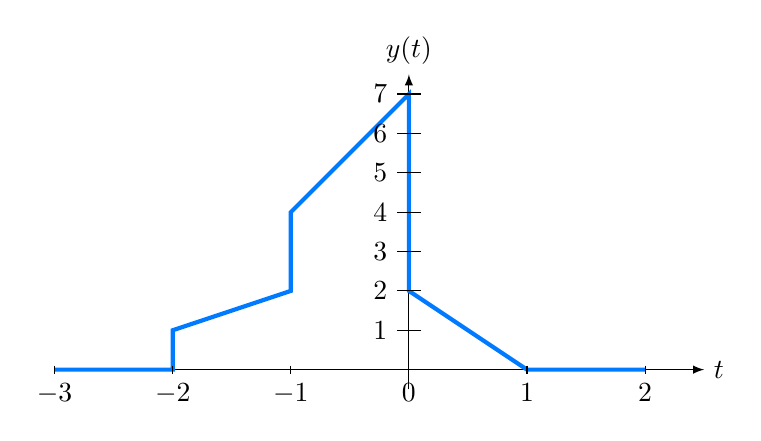
\begin{tikzpicture}[>=latex, yscale=0.5, xscale=1.5]
        \draw[->] (-3,0) -- (2.5, 0) node[right] {$t$};
        \draw[->] (0,-0.5) -- (0,7.5) node[above] {$y(t)$};
        \draw[lightblue, line width=1.5] (-3,0) -- (-2,0) -- (-2,1) -- (-1,2) -- (-1, 4) -- (0,7) -- (0,2) -- (1,0) -- (2,0);
        \foreach \x in {-3, -2, ..., 2} {\draw (\x,0.1) -- (\x,-0.1) node[below] {$\x$};}
          \foreach \y in {1,...,7} {\draw (0.1,\y) -- (-0.1,\y) node[left] {$\y$};}
      \end{tikzpicture}
    \end{center}
  \item \lb{Sean \[
  x(t)=\begin{cases}
    1, & 0\le t\le 1\\
    0,  & \text{otro valor}
  \end{cases}\qquad h(t)=x\left( \dfrac{t}{\alpha} \right),\text{ donde $0<\alpha\le 1$ }
  \] } 
  \begin{enumerate}[label=\color{red}\textbf{\alph*)}]
    \item \db{Determine y esboce $y(t)=x(t)\ast h(t)$.}
    \item \db{Si $\dfrac{\mathrm{d}y(t)}{\dt}$ contiene sólo tres discontinuidades, ¿cuál es el valor de $\alpha$?} 
  \end{enumerate}
\item \lb{Sean \[
x(t)=u(t-3)-u(t-5)\qquad h(t)=e^{-3t} u(t)
\] } 
\begin{enumerate}[label=\color{red}\textbf{\alph*)}]
  \item \db{Calcule $y(t)=x(t)\ast h(t)$} 
  \item \db{Calcule $g(t)=\dfrac{\mathrm{d}x(t)}{\dt}\ast h(t)$} 
  \item \db{Establece una relación entre $g(t)$ e $y(t)$} 
\end{enumerate}
\item \lb{Calcule la convolución de los siguientes pares de señales:}
  \begin{enumerate}[label=\color{red}\textbf{\alph*)}]
    \item \db{$x[n]=\alpha^nu[n],\quad h[n]=\beta^nu[n],\quad \alpha\neq \beta$} 
    \item \db{$x[n]=h[n]=\alpha^nu[n]$} 
    \item \db{$x[n]=\left( -\dfrac{1}{2} \right) ^{n}u[n-4],\quad h[n]=4^nu[2-n]$} 
    \item \db{$x[n]=2^nu[-n],\quad h[n]=u[n]$}
  \end{enumerate}
\item \lb{¿Cuál/es de las siguientes respuestas al impulso corresponden a sistemas LTI estables?} 
  \begin{enumerate}[label=\color{red}\textbf{\alph*)}]
    \item \db{$h(t)=e^{-(1-2j)t}u(t) $} 
    \item \db{$h(t)=e^{-t}\cos(2t)u(t) $} 
  \end{enumerate}
\item \lb{¿Cuál/es de las siguientes respuestas al impulso corresponden a sistemas LTI estables?} 
  \begin{enumerate}[label=\color{red}\textbf{\alph*)}]
    \item \db{$h[n]=n\cos\left( \dfrac{\pi}{4} \right) $} 
    \item \db{$h[n]=3^nu[-n+10]$} 
  \end{enumerate}
\item \lb{Para las siguientes respuestas al impulso de sistemas LTI, determine si cada sistema es causal y/o estable, justificando la respuesta.}
  \begin{enumerate}[label=\color{red}\textbf{\alph*)}]
    \item \db{$h[n]=\left( \dfrac{1}{5} \right) ^nu[n]$} 
    \item \db{$h[n]=0.8^nu[n+2]$} 
    \item  \db{$h[n]=\left( \dfrac{1}{2} \right) ^n u[-n]$} 
    \item \db{$h[n]=5^nu[3-n]$} 
    \item \db{$h[n]=\left( -\dfrac{1}{2} \right) ^nu[n]+1.01^nu[n-1]$} 
    \item \db{$h[n]=\left( -\dfrac{1}{2} \right) ^nu[n]+1.01^nu[1-n]$} 
    \item \db{$h[n]=n\left( \dfrac{1}{3} \right) ^nu[n-1]$} 
  \end{enumerate}
\item \lb{Considere un sistema LTI que se encuentra incialmente en reposo y cuya entrada $x(t)$ y salida $y(t)$ se relacionan por la ecuación diferencial \[
\dfrac{\mathrm{d}}{\dt}y(t)+4y(t)=x(t)
\] } 
\begin{enumerate}[label=\color{red}\textbf{\alph*)}]
  \item \db{Obtenga la respuesta al impulso del sistema.}
  \item \db{Si $x(t)=e^{(-1+3j)t} u(t)$, calcule $y(t)$} 
\end{enumerate}
\item \lb{Considere un sistema LTI que se encuentra inicialmente en reposo y cuya entrada  $x(t)$ y salida  $y(t)$ se relacionan por la ecuación diferencial  \[
\dfrac{\mathrm{d}}{\dt}y(t)+3y(t)=2x(t)
\] } 
\begin{enumerate}[label=\color{red}\textbf{\alph*)}]
  \item \db{Si $x(t)=\cos(2t)u(t)$, calcule $y(t)$.}
  \item \db{Obtenga la respuesta al impulso del sistema.} 
\end{enumerate}
\item \lb{Obtenga la respuesta al impulso, así como las propiedades de memoria, causalidad, estabilidad, invarianza en el tiempo y linealidad de los siguientes sistemas:}
  \begin{enumerate}[label=\color{red}\textbf{\alph*)}]
    \item \db{$y(t)=\int_{-\infty}^{t} x(\tau)\mathrm{d}\tau $} 
    \item \db{$y(t)=\int_{-\infty}^{t} 2x(\tau-5)\mathrm{d}\tau $} 
    \item \db{$y(t)=\int_{-\infty}^{t} e^{-(t-\tau)} 3x(\tau-2)\mathrm{d}\tau $} 
    \item \db{$y(t)=\int_{t-3}^{t+2} e^{-(t+\tau)} x(\tau-2)\mathrm{d}\tau $} 
  \end{enumerate}
\item \lb{Un sistema discreto viene determinado por la relación entrada-salida \[
      y[n]=e^{j\frac{2\pi}{10} (n+2)}x[n-2]. 
\] Analice las propiedades de memoria, causalidad, estabilidad, invarianza en el tiempo y linealidad del sistema.}
\item \lb{Considere la señal $x[n]=\bigwedge\left( \dfrac{n}{4} \right) +\prod\left( \dfrac{n-2}{5} \right) $. Obtenga y represente la parte par e impar de esta señal. Calcule la energía y potencia de $x[n]$, indicando si se trata de una señal defindia en energía o en potencia.}

\item \lb{Calcule la convolución de las señales \[
      x_1[n]=(n-6)\prod\left( \dfrac{n-6}{13} \right) \qquad x_2[n]=\prod\left( \dfrac{-n-3}{5} \right) 
\] \underline{Nota:} la suma de una progresión aritmética $a_{n_i}, a_{n_i+1},\dots,a_{n_f}$, con $a_{n_i+1}=a_{n_i}+d,a_{n_i+2}=a_{n_i}+2d,\dots$ es \[
\sum_{k=n_i}^{n_f} a_k=\dfrac{(n_f-n_i+1)(a_{n_i}+a_{n_f})}{2}.
\] } 
\end{enumerate}
\end{document}
